
\section{WENO methods, nonlinear equations, and flux-splitting}
\label{sec:weno-burgers-fvs}

%\todo{This shouldn't go here - probably belongs after the Euler section - but for now this keeps all the WENO stuff together}
%\todo{Also note that I haven't followed the notation of the rest of the notes as I was too lazy to work out what it was.}

For a nonlinear scalar conservation law
\begin{equation}
  \label{eq:scalar_conslaw}
  u_t + f(u)_x = 0
\end{equation}
the WENO method introduced in section~\ref{sec:ho-intro} above does not work,
as we have assumed the characteristic
information travels in one direction only. We have also reconstructed the
variable $q$ and from that constructed the ``flux'' which we feed into the
differencing formula of equation~\eqref{sec:ho-fd} to update the solution: this
will not work either.

In the nonlinear case, we instead reconstruct the \emph{flux} directly. That
is, given the state $u_i$ at location $x_i$, we compute the flux $f_i = f(u_i)$
and reconstruct the flux $f_{i+\myhalf}$ using the WENO reconstruction above.

This has the significant problem that we have no characteristic information for
the flux: does it propagate to the left or to the right? To get around this we
introduce \emph{flux splitting}. We write
\begin{equation}
  \label{eq:flux-splitting}
  f(u) = f^{(+)}(u) + f^{(-)}(u)
\end{equation}
where we choose the functions such that the information contained in $f^{(+)}$
propagates to the right and that in $f^{(-)}$ propagates to the left. There are
many ways of doing this, but the simplest is the \emph{Lax-Friedrichs} flux
splitting
\begin{equation}
  \label{eq:lf-flux-split}
  f^{(\pm)}(u) = \tfrac{1}{2} \left( f(u) \pm \alpha u \right)
\end{equation}
where $\alpha \ge \max | \partial_u f |$. With $\alpha$ being larger than the maximum propagation speed, this means that
\begin{equation}
  \label{eq:lf-flux-split-speeds}
  \partial_u f^{(+)} \ge 0, \quad \partial_u f^{(-)} \le 0,
\end{equation}
and the characteristic information contained in $f^{(\pm)}$ will propagate as required.

The simplest flux-split algorithm is then
\begin{enumerate}
  \item Compute the maximum characteristic speed $\alpha$ over the entire computational grid;
  \item Compute the split fluxes $f^{(\pm)}$ from equation~\eqref{eq:lf-flux-split};
  \item Reconstruct $f^{(+)}$ to the right using, e.g., the WENO algorithm of section~\ref{sec:WENO};
  \item Reconstruct $f^{(-)}$ to the left using the same method;
  \item Compute $f_{i+\myhalf} = f^{(+)}_{i+\myhalf} + f^{(-)}_{i+\myhalf}$;
  \item Update the state using equation~\eqref{eq:consup}.
\end{enumerate}

\begin{figure}[t]
\centering
% figure generated by hydro_examples/advection/weno.py
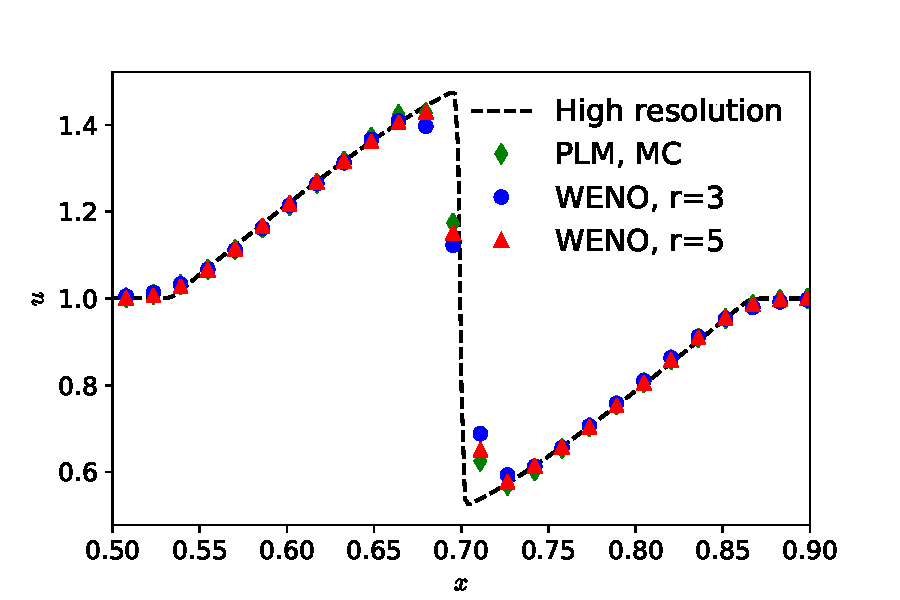
\includegraphics[width=0.8\linewidth]{weno-vs-plm-burger}
\caption[Comparing PLM and WENO methods for Burgers' equation]
{\label{fig:weno-vs-plm-burger} Numerical solutions to Burgers' equation using the piecewise linear method as in figure~\ref{fig:burgers-shock} and two flux-split WENO methods as outlined in section~\ref{sec:weno-burgers-fvs}. This uses the same sinusoidal data as figure~\ref{fig:burgers-shock} shortly after shock formation. Note that the WENO methods are not obviously any better at resolving the shock than the simpler piecewise linear approach.\\
\hydroexdoit{\href{https://github.com/zingale/hydro_examples/blob/master/advection/weno_burgers.py}{weno_burgers.py}}}
\end{figure}
%

As a direct comparison between the piecewise linear method used at the start of
this chapter, and the more complex WENO methods introduced here, we start with
looking at a shock forming from smooth initial data. Figure~\ref{fig:weno-vs-plm-burger}}
shows the evolution of the sinusoidal initial data as used in figure~\ref{fig:burgers-shock},
but only showing the result at one time, shortly after characteristic crossing
leads to a shock. We see that there is very little difference between the
different numerical methods. The characteristic focusing means that all the
methods have a similar number of points within the shock. The piecewise linear
method appears to capture the edges of the shock slightly more accurate than the
(higher order) WENO method with $r=3$. This is likely as the piecewise linear
method is using the exact solution to the Riemann Problem, whilst the WENO method
is using the more diffusive Lax-Friedrichs flux splitting. At the higher $r=5$
order there is a marginal advantage to the WENO method.

\begin{figure}[t]
\centering
% figure generated by hydro_examples/advection/weno.py
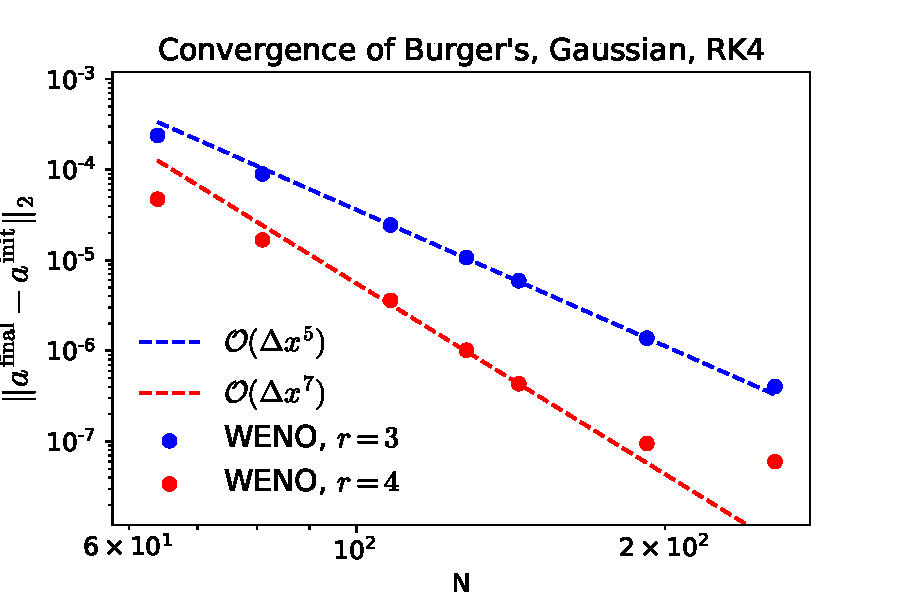
\includegraphics[width=0.8\linewidth]{weno-converge-burgers}
\caption[WENO convergence rates for Burgers' equation]
{\label{fig:weno-converge-burgers} WENO solutions from evolving Burgers'
equation for an initial Gaussian profile, stopping before the solution is
discontinuous. A fourth order Runge-Kutta method is used for time evolution.
For $r=3$ we see the expected fifth ($2 r - 1$) order convergence.
For $r=5$ we see seventh order convergence briefly, before the error from the
time integrator dominates. \\
\hydroexdoit{\href{https://github.com/zingale/hydro_examples/blob/master/advection/weno_burgers.py}{weno_burgers.py}}}
\end{figure}
%

The advantages of the WENO method arise when the profile is still continuous, as
in the rarefaction problem, or at times before shocks have formed. To confirm
that high-order convergence is still possible for a nonlinear problem, an
initially Gaussian profile is evolved for a short time and compared to the
exact solution (computed from characteristic tracing). The resulting error
convergence is shown in figure~\ref{fig:weno-converge-burgers}. We see the
expected fifth and seventh order convergence rates, at least for some of the
resolutions. At too low a resolution the higher order terms in the error
expansion affect the solution. At too high a resolution, for the higher-order
method, the time integration error starts to dominate.

\subsection{Extensions}

Extending to multiple dimensions using dimensional splitting. From the
finite-difference form there are no transverse Riemann problems to solve. From
using the Method of Lines there is no issue about ordering the dimensional
sweeps: the updates in each direction are computed separately but applied
together in the time integrator. This formally retains the high-order accuracy
but can lose significant absolute accuracy -- compare the advection of a
top-hat function with lower order methods using transverse Riemann problem
solutions.

The global Lax-Friedrichs flux splitting above can be excessively diffusive. A
local Lax-Friedrichs flux splitting, where $\alpha$ is computed at each point
by maximising over the characteristic speed within the stencil at that point, is
less diffusive but slightly more expensive. Roe-style flux splittings are
possible but not always stable.

When dealing with nonlinear systems the flux split method generalizes directly.
The simplest method is to compute $\alpha$ by maximizing over all
characteristics. It is possible to significantly reduce the diffusive nature of
the flux splitting by reconstructing the \emph{characteristic} fluxes and using
a local computational of the specific characteristic speed. This requires both
significant additional computational expense and the knowledge of the spectral
information (left and right eigenvectors of the Jacobian matrix).
